\chapter{State of the Art}

The first part of this chapter (\autoref{section:background}) provides the theoretical background for this thesis. First, we will discuss the field of multi-robot systems, providing the reader with an understanding of how the field has evolved and how it may further evolve. Next, we examine RobotWeb \cite{Robotweb}, the research that this thesis seeks to build upon. Finally, we discuss various security issues present in the field to arrive at the research question for this thesis. 

The second part of this chapter (\autoref{section:related_work}) evaluates several different techniques that have been proposed to solve the aforementioned security issues. We will first consider the ``Wifi-Fingerprinting'' technique which uses the physical characteristics of signal propagation in networks to prevent attacks. Then we will consider techniques using the ``Proof of Work'' algorithm to deter attackers.

The final part of this chapter (\autoref{section:prelim}) concludes with an overview of the preliminaries present at the start of this thesis.

\section{Multi-Robot Systems} \label{section:background}
The study of multi-robot systems concerns itself with studying how to allow multiple robots to operate in the same environment \cite{MRS-Implicit-Explicit-Comms}. Multi-robot systems have several advantages over single-robot systems; they are more effective, efficient, flexible, and resilient \cite{MultiVsSingleRobotSystems}. These robots can behave competitively or collaboratively, coordinate statically or dynamically, communicate explicitly or implicitly, consist of homogeneous or heterogeneous robots, and make decisions centrally or decentrally \cite{MultiRobotCoordinationSurvey}.

\subsection{Competitive vs Collaborative Behavior}
Multiple robots which share a common goal are considered to be behaving collaboratively, whereas if each robot aimed to complete its own goal at the expense of all others, it would be said to be behaving competitively \cite{MultiRobotCoordinationSurvey}. Examples of collaboration range from teams of robots constructing a lunar habitat \cite{LunarHabitatConstructionExample} to exploring unknown environments \cite{MultiRobotExplorationExample}.

\subsection{Static vs Dynamic Coordination}
If a multi-robot system operates using a set of predetermined rules, then it can be said to be coordinating itself statically. A possible set of rules would be that each robot must maintain a certain distance between it and all others. Dynamically coordinated multi-robot systems would instead make decisions whilst performing the task and may communicate to do so \cite{MultiRobotCoordinationSurvey}.

\subsection{Explicit vs Implicit Communication}
Most multi-robot systems communicate explicitly by sending messages to each other via a hardware communication interface, for example, a wifi module \cite{MultiRobotCoordinationSurvey}. However, there is still a sizeable minority of approaches that send messages through their environment (implicit communication) and rely on others to sense these messages to receive them. An example of implicit communication is found in \cite{FootballRobots}, where the authors use it to allow a team of robots to play a game of football for the RoboCup Simulation League \cite{RoboCup}.

\subsection{Homogeneous vs Heterogeneous Robots}
Multi-robot systems can either contain robots with identical hardware, which are known as homogeneous systems, or individual robots may have different hardware, making them heterogeneous systems. Heterogeneous systems allow a greater degree of specialisation within a multi-robot system but also add additional decision-making complexity.

\subsection{Centralised vs Decentralised Decision Making}
A multi-robot system is said to have centralised decision-making if all robots communicate with a central agent, which may or may not be a robot itself, to receive instructions. Centralised schemes perform better with smaller groups of robots and in static environments, they also introduce a single point of failure in the central agent \cite{MultiRobotCoordinationSurvey}. Decentralised schemes, however, avoid vesting authority into a central agent and instead treat each agent as an equal part of the system, which allows them to avoid the problems associated with centralised schemes. However, decentralised schemes lose the guarantee that they will converge to an optimal solution, as decisions are made with incomplete information. % Should I add more citations here?
In addition to centralised and decentralised schemes, multi-robot systems may also be organised in a hierarchical manner, where some robots would be chosen as local leaders, but no global leader would exist.

\section{Robot Web}
This thesis seeks to build upon the work done in ``A Robot Web for Distributed Many-Device Localisation'' \cite{Robotweb}, which describes a method for \textit{heterogeneous} robots in a \textit{decentralised} multi-robot system to \textit{collaborate} via \textit{explicit communication} to localise \textit{dynamically}.

Robots in the Robot Web move along predefined paths, estimating their location via internal odometry. When a robot senses another, it communicates its measurement to the other robot, and then both robots use the measurement to update their location estimates. Since we live in an imperfect world, each sensor measurement carries with it a small amount of noise, which is reflected in the Robot Web by a degree of uncertainty attached to each robot's location estimate and represented by a Gaussian distribution.

This section will introduce the reader to the core concepts used in the Robot Web and assemble them to provide the reader with an understanding of how the Robot Web functions and some of its limitations.

\subsection{Factor Graphs} 
A factor graph is an undirected bipartite graph used to represent the factorisation of a probability distribution $p(X)$. A probability distribution can be said to be factorised if it is written in the form:

\begin{equation}
p(X) = \underset{i}{\prod} f_i(X_i)
\end{equation}

The nodes of a factor graph can either represent variables ($X_i$) or factors ($f_i$). There are several different ways to draw factor graphs, but we will use the one defined in \cite{FactorGraphDrawingFormat}, where factors are drawn as squares and variables are drawn as circles.

\begin{figure}[!h]
    \centering
    

\tikzset{every picture/.style={line width=0.75pt}} %set default line width to 0.75pt        

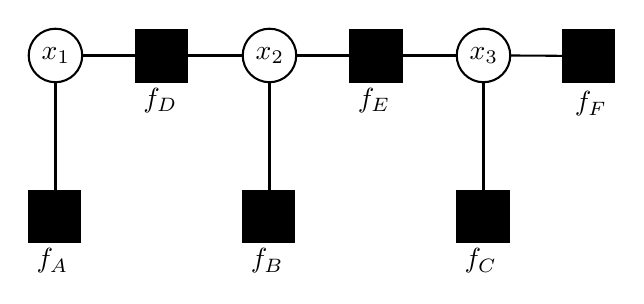
\begin{tikzpicture}[x=0.75pt,y=0.75pt,yscale=-1,xscale=1]
%uncomment if require: \path (0,288); %set diagram left start at 0, and has height of 288

%Shape: Square [id:dp542094098374186] 
\draw  [fill={rgb, 255:red, 0; green, 0; blue, 0 }  ,fill opacity=1 ] (86.34,228.71) -- (110.92,228.71) -- (110.92,253.29) -- (86.34,253.29) -- cycle ;
%Shape: Rectangle [id:dp9431678202688636] 
\draw  [fill={rgb, 255:red, 0; green, 0; blue, 0 }  ,fill opacity=1 ] (189.45,228.71) -- (214.03,228.71) -- (214.03,253.29) -- (189.45,253.29) -- cycle ;
%Shape: Rectangle [id:dp5515594438313509] 
\draw  [fill={rgb, 255:red, 0; green, 0; blue, 0 }  ,fill opacity=1 ] (292.57,228.71) -- (317.14,228.71) -- (317.14,253.29) -- (292.57,253.29) -- cycle ;
%Shape: Rectangle [id:dp19402149967725735] 
\draw  [fill={rgb, 255:red, 0; green, 0; blue, 0 }  ,fill opacity=1 ] (137.9,151.38) -- (162.47,151.38) -- (162.47,175.96) -- (137.9,175.96) -- cycle ;
%Shape: Rectangle [id:dp9723919948872586] 
\draw  [fill={rgb, 255:red, 0; green, 0; blue, 0 }  ,fill opacity=1 ] (241.01,151.38) -- (265.59,151.38) -- (265.59,175.96) -- (241.01,175.96) -- cycle ;
%Shape: Circle [id:dp9001944284946917] 
\draw   (86,163.41) .. controls (86,156.29) and (91.77,150.52) .. (98.89,150.52) .. controls (106.01,150.52) and (111.78,156.29) .. (111.78,163.41) .. controls (111.78,170.53) and (106.01,176.3) .. (98.89,176.3) .. controls (91.77,176.3) and (86,170.53) .. (86,163.41) -- cycle ;
%Shape: Ellipse [id:dp029985916423680425] 
\draw   (189.11,163.41) .. controls (189.11,156.29) and (194.88,150.52) .. (202,150.52) .. controls (209.12,150.52) and (214.89,156.29) .. (214.89,163.41) .. controls (214.89,170.53) and (209.12,176.3) .. (202,176.3) .. controls (194.88,176.3) and (189.11,170.53) .. (189.11,163.41) -- cycle ;
%Shape: Ellipse [id:dp8505763078012687] 
\draw   (292.22,163.41) .. controls (292.22,156.29) and (297.99,150.52) .. (305.11,150.52) .. controls (312.23,150.52) and (318,156.29) .. (318,163.41) .. controls (318,170.53) and (312.23,176.3) .. (305.11,176.3) .. controls (297.99,176.3) and (292.22,170.53) .. (292.22,163.41) -- cycle ;
%Straight Lines [id:da5591298719832298] 
\draw    (202,176.3) -- (202,236.1) ;
%Straight Lines [id:da8657801799701208] 
\draw    (305.11,176.3) -- (305.11,236.1) ;
%Straight Lines [id:da7323179142438296] 
\draw    (98.89,176.3) -- (98.89,236.1) ;
%Straight Lines [id:da2650402956705291] 
\draw    (141.85,163.41) -- (111.78,163.41) ;
%Straight Lines [id:da6929917679064295] 
\draw    (189.11,163.41) -- (159.04,163.41) ;
%Straight Lines [id:da7044874759875848] 
\draw    (244.96,163.41) -- (214.89,163.41) ;
%Straight Lines [id:da30371490539779855] 
\draw    (292.22,163.41) -- (262.15,163.41) ;
%Shape: Rectangle [id:dp26239558807935515] 
\draw  [fill={rgb, 255:red, 0; green, 0; blue, 0 }  ,fill opacity=1 ] (343.59,151.38) -- (368.16,151.38) -- (368.16,175.96) -- (343.59,175.96) -- cycle ;
%Straight Lines [id:da46629291479421253] 
\draw    (355.87,163.67) -- (318,163.41) ;


% Text Node
\draw (90.75,157.95) node [anchor=north west][inner sep=0.75pt]    {$x_{1}$};
% Text Node
\draw (193.86,157.95) node [anchor=north west][inner sep=0.75pt]    {$x_{2}$};
% Text Node
\draw (296.97,157.95) node [anchor=north west][inner sep=0.75pt]    {$x_{3}$};
% Text Node
\draw (88.3,255) node [anchor=north west][inner sep=0.75pt]    {$f_{A}$};
% Text Node
\draw (191.48,255) node [anchor=north west][inner sep=0.75pt]    {$f_{B}$};
% Text Node
\draw (294.53,255) node [anchor=north west][inner sep=0.75pt]    {$f_{C}$};
% Text Node
\draw (243.04,177.67) node [anchor=north west][inner sep=0.75pt]    {$f_{E}$};
% Text Node
\draw (139.79,177.67) node [anchor=north west][inner sep=0.75pt]    {$f_{D}$};
% Text Node
\draw (347.59,179.36) node [anchor=north west][inner sep=0.75pt]    {$f_{F}$};


\end{tikzpicture}


    \caption[Example factor graph]{An example of a factor graph}
\end{figure}

The above factor graph represents the following factorisation:

\begin{equation}
    p(X_1, X_2, X_3) = f_A(X_1)f_B(X_2)f_C(X_3)f_D(X_1, X_2)f_E(X_2, X_3)f_F(X_3)
    \label{eqn:factors}
\end{equation}

Assuming that each variable takes discrete values, suppose we wanted to find the probability that $X_1 = z$ for some value of $z$ using the above factor graph. Then we would need to find:

\begin{equation}
    p(X_1 = z, X_2, X_3) = \underset{i=X_2}{\sum} \underset{j=X_3}{\sum} p(X_1 = z, X_2 = i, X_3 =j)
    \label{eqn:bp_derivation_1}
\end{equation}

And by \ref{eqn:factors} we get:

\begin{equation}
    p(X_1 = z, X_2, X_3) = \underset{i=X_2}{\sum} \underset{j=X_3}{\sum} f_A(z)f_B(i)f_C(j)f_D(z, i)f_E(z, j)f_F(j)
\end{equation}


which can be rearranged to form:

\begin{equation}
    p(X_1 = z, X_2, X_3) = f_A(z) \underset{i=X_2}{\sum} \left(f_D(z, i)f_B(i) \left(\underset{j=X_3}{\sum} f_E(z, j)f_C(j)f_F(j) \right)\right)
    \label{eqn:x1}
\end{equation}

Similarly, if we wanted to find the probability that $X_2 = z$ for some z we would need to find:

\begin{equation}
    p(X_1, X_2 = z, X_3) = f_b(z) \left(\underset{i=X_1}{\sum} f_D(i, z) f_A(i)\right) \left(\underset{j=X_3}{\sum} f_E(z, j) f_C(j) f_F(j)\right)
    \label{eqn:x2}
\end{equation}

Noticing how the sum over $X_3$ in both \ref{eqn:x1} and \ref{eqn:x2} is the same, we may want to ``cache'' the result when dealing with large factor graphs, to improve performance. To do this we can associate calculations with nodes in the factor graph. We call these associations ``messages''.

The general form of a message from variable $i$ to factor $j$ is the product of the messages from all other neighbouring factors \cite{GaussianBP}. Put formally:

\begin{equation}
    m_{x_i \rightarrow f_j} = \underset{s \in N(i) \backslash j }{\prod} m_{f_s \rightarrow x_i}
    \label{eqn:v_f}
\end{equation}

The general form of a message from factor $j$ to variable $i$ is the product of the messages from all other neighbouring variables and the factor applied to all other variables except $i$ \cite{GaussianBP}. Put formally:

\begin{equation}
    m_{f_j \rightarrow x_i} = \left(\underset{X_j \backslash x_i}{\sum} f_j(X_j)\right) \left(\underset{k \in N(j) \backslash i}{\prod} m_{x_k \rightarrow f_j}\right)
    \label{eqn:f_v}
\end{equation}

Finally, the marginal value of a variable is simply the product of all incoming messages to it \cite{GaussianBP}.

\begin{equation}
    p(x_i) = \underset{s \in N(i)}{\prod} m_{f_s \rightarrow x_i}
    \label{eqn:bp_belief}
\end{equation}

\subsection{Belief Propagation}
The above equations are used by the Belief Propagation algorithm, an iterative message-passing algorithm used to calculate the marginal value for each variable in a factor graph \cite{GaussianBP}. Each iteration of Belief Propagation has 3 phases:

\begin{enumerate}
    \item Variables send messages to each of their neighbouring factors \ref{eqn:v_f}.
    \item Factors send messages to each of their neighbouring variables \ref{eqn:f_v}.
    \item Each variable updates its ``belief'' (its estimated marginal value) \ref{eqn:bp_belief}.
\end{enumerate}

The original Belief Propagation algorithm was designed to be used in tree-like graphs, i.e. graphs without loops \cite{GaussianBP}. However, empirical evidence has shown that ``Loopy-BP'' can still converge to provide useful results in a variety of problem domains \cite{GaussianBP}. % TODO replace citations with better ones 

\subsection{Gaussian Belief Propagation}
A special case of the Belief Propagation algorithm is Gaussian Belief Propagation (henceforth referred to as GBP), which applies to problems where all variables follow a Gaussian distribution, and all factors are Gaussian functions of their inputs.

Under Gaussian Belief Propagation, each message can be interpreted as a Gaussian and so must contain sufficient information to produce one. A naive way of achieving this is to include a mean vector and a covariance matrix in each message. However, this approach is computationally expensive as it requires a full matrix multiplication whenever messages are multiplied which is an order $O(n^3)$ operation. An alternative approach is to use the \textit{canonical form} of the multivariate Gaussian distribution.

The canonical form uses an \textit{information vector} ($\eta$) and a \textit{precision matrix} ($\Lambda$) defined as follows:
\begin{eqnarray}
	\eta = \Sigma^{-1} \mu&
	\Lambda = \Sigma^{-1} \label{eqn:canonical}
\end{eqnarray}

where $\Sigma$ is the covariance matrix and $\mu$ is the mean vector. Now multiplying messages is made more efficient as it only requires the addition of both messages' $\eta$ and $\Lambda$ values (\autoref{eqn:gbp-sum}), making it an order $O(n^2)$ operation in the worst case. A further performance improvement can be made by recognising that the precision matrix is a sparse matrix \cite{GaussianBP}.
\begin{eqnarray}
	\eta_I = \underset{i \in I}{\sum} \eta_i &
	\Lambda_I = \underset{i \in I}{\sum} \Lambda_i \label{eqn:gbp-sum}
\end{eqnarray}

\subsection{Lie Theory}
Lie theory is a subset of group theory focused on studying \textit{Lie groups}. Lie theory is a vast and abstract field, from which we only need to borrow a few concepts. The first is that positions and rotations can be represented as Lie groups, for example, the group $SO2$ represents a rotation in 2D space and the $SE3$ group represents a rigid motion in 3D space. The second core concept is the \textit{tangent space} which allows small deviations to be applied to the Lie group uniformly regardless of the value it operates on. This concludes our whirlwind tour of Lie theory, we invite the reader to read \cite{MicroLieTheory} for a more detailed tutorial.

% QUESTION: Do I need this at all?
% A group is a set of elements $G$ combined with a composition operation $\circ$, such that the following properties hold:
% \begin{enumerate}
%     \item Composing 2 elements of G results in another element of G
%     \item There exists an identity element $\epsilon$ so that composing any element with $\epsilon$ or $\epsilon$ with any element results in the same element
%     \item Composing an element with its inverse results in $\epsilon$
%     \item Composition is associative
% \end{enumerate}

% A Lie group is a group combined with a smooth manifold

\subsection{Putting it all together}
Now that we have covered all of the prerequisites to understanding how the Robot Web operates, we shall now demonstrate how they can be assembled into the Robot Web.

Every robot in the Robot Web needs to estimate its current location and bearing at all times, this process is called localisation. One simple localisation method is to use odometry, which uses internal sensors to measure its displacement from its previous localisation. Since no sensor is perfect, this introduces a small amount of noise, which can be accurately modelled using a Gaussian distribution. The Robot Web simulates odometry using a factor graph, each known position of the robot maps to a pose variable, and the variables of each pair of successive positions are connected by an odometry factor. On every timestep, the robot performs several iterations of Gaussian Belief Propagation to estimate its current localisation.

The Robot Web further improves the accuracy of robots' localisations by allowing robots to measure each other using external sensors. When a robot senses another, it creates a factor in its factor graph between its and the other's latest pose variables. When each robot wants to send a message to another, it publishes the message to its \textbf{Robot Web Page}, which the other robot will eventually read and use to update its localisation.

We can group the messages sent by one robot to another into two categories; the robot will either send its belief of its localisation, or its belief of the other's localisation. The first type of message is sent when the factor connecting the sender to the receiver, was created by the receiver, we call this a \textit{response}. The second type of message is sent when the connecting factor was created by the sender, we call this a \textit{request}. 

\begin{figure}[!h]
    \centering
    

\tikzset{every picture/.style={line width=0.75pt}} %set default line width to 0.75pt        

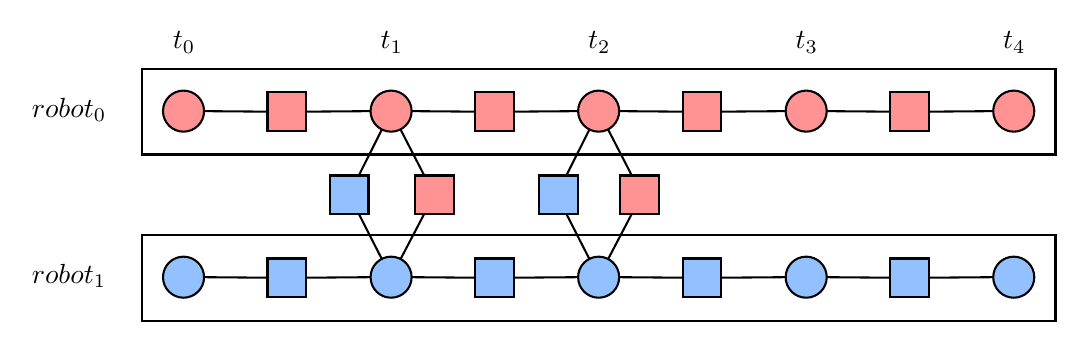
\begin{tikzpicture}[x=0.75pt,y=0.75pt,yscale=-1,xscale=1]
%uncomment if require: \path (0,288); %set diagram left start at 0, and has height of 288

%Straight Lines [id:da47036734988196627] 
\draw    (299.67,170.04) -- (319.89,209.71) ;
%Straight Lines [id:da6881382794521629] 
\draw    (319.89,129.71) -- (299.67,170.04) ;
%Straight Lines [id:da3959117741800886] 
\draw    (319.89,129.71) -- (340.67,170.04) ;
%Straight Lines [id:da6282284807536171] 
\draw    (340.67,170.04) -- (319.89,209.71) ;
%Straight Lines [id:da5198960712037324] 
\draw    (199.67,170.04) -- (219.89,209.71) ;
%Straight Lines [id:da8902598554725618] 
\draw    (219.89,129.71) -- (199.67,170.04) ;
%Straight Lines [id:da2738660568678817] 
\draw    (219.89,129.71) -- (240.67,170.04) ;
%Straight Lines [id:da06728554169051759] 
\draw    (240.67,170.04) -- (219.89,209.71) ;
%Straight Lines [id:da34036055728120096] 
\draw [fill={rgb, 255:red, 255; green, 147; blue, 147 }  ,fill opacity=1 ]   (329.78,129.71) -- (369.67,130.04) ;
%Straight Lines [id:da8072322510197338] 
\draw [fill={rgb, 255:red, 255; green, 147; blue, 147 }  ,fill opacity=1 ]   (369.67,130.04) -- (410,129.71) ;
%Straight Lines [id:da405451058550087] 
\draw [fill={rgb, 255:red, 255; green, 147; blue, 147 }  ,fill opacity=1 ]   (429.78,129.71) -- (469.67,130.04) ;
%Straight Lines [id:da7616794610228106] 
\draw [fill={rgb, 255:red, 255; green, 147; blue, 147 }  ,fill opacity=1 ]   (469.67,130.04) -- (510,129.71) ;
%Straight Lines [id:da6814419083610201] 
\draw [fill={rgb, 255:red, 255; green, 147; blue, 147 }  ,fill opacity=1 ]   (229.78,129.71) -- (269.67,130.04) ;
%Straight Lines [id:da7724102331322766] 
\draw [fill={rgb, 255:red, 255; green, 147; blue, 147 }  ,fill opacity=1 ]   (269.67,130.04) -- (310,129.71) ;
%Straight Lines [id:da5821529621200299] 
\draw [fill={rgb, 255:red, 255; green, 147; blue, 147 }  ,fill opacity=1 ]   (169.67,130.04) -- (210,129.71) ;
%Straight Lines [id:da0542087989667579] 
\draw [fill={rgb, 255:red, 255; green, 147; blue, 147 }  ,fill opacity=1 ]   (129.78,129.71) -- (169.67,130.04) ;
%Shape: Square [id:dp4499442483222458] 
\draw  [fill={rgb, 255:red, 255; green, 147; blue, 147 }  ,fill opacity=1 ] (160.34,120.71) -- (179,120.71) -- (179,139.37) -- (160.34,139.37) -- cycle ;
%Shape: Circle [id:dp2600881142320077] 
\draw  [fill={rgb, 255:red, 255; green, 147; blue, 147 }  ,fill opacity=1 ] (110,129.71) .. controls (110,124.25) and (114.43,119.82) .. (119.89,119.82) .. controls (125.35,119.82) and (129.78,124.25) .. (129.78,129.71) .. controls (129.78,135.17) and (125.35,139.6) .. (119.89,139.6) .. controls (114.43,139.6) and (110,135.17) .. (110,129.71) -- cycle ;
%Shape: Rectangle [id:dp7305091073359651] 
\draw   (100,109.6) -- (540,109.6) -- (540,150.6) -- (100,150.6) -- cycle ;
%Shape: Square [id:dp49665350033925293] 
\draw  [fill={rgb, 255:red, 255; green, 147; blue, 147 }  ,fill opacity=1 ] (260.34,120.71) -- (279,120.71) -- (279,139.37) -- (260.34,139.37) -- cycle ;
%Shape: Circle [id:dp8551402235390253] 
\draw  [fill={rgb, 255:red, 255; green, 147; blue, 147 }  ,fill opacity=1 ] (210,129.71) .. controls (210,124.25) and (214.43,119.82) .. (219.89,119.82) .. controls (225.35,119.82) and (229.78,124.25) .. (229.78,129.71) .. controls (229.78,135.17) and (225.35,139.6) .. (219.89,139.6) .. controls (214.43,139.6) and (210,135.17) .. (210,129.71) -- cycle ;
%Shape: Square [id:dp6259568957324568] 
\draw  [fill={rgb, 255:red, 255; green, 147; blue, 147 }  ,fill opacity=1 ] (360.34,120.71) -- (379,120.71) -- (379,139.37) -- (360.34,139.37) -- cycle ;
%Shape: Circle [id:dp7516686593765485] 
\draw  [fill={rgb, 255:red, 255; green, 147; blue, 147 }  ,fill opacity=1 ] (310,129.71) .. controls (310,124.25) and (314.43,119.82) .. (319.89,119.82) .. controls (325.35,119.82) and (329.78,124.25) .. (329.78,129.71) .. controls (329.78,135.17) and (325.35,139.6) .. (319.89,139.6) .. controls (314.43,139.6) and (310,135.17) .. (310,129.71) -- cycle ;
%Shape: Square [id:dp4907257696393781] 
\draw  [fill={rgb, 255:red, 255; green, 147; blue, 147 }  ,fill opacity=1 ] (460.34,120.71) -- (479,120.71) -- (479,139.37) -- (460.34,139.37) -- cycle ;
%Shape: Circle [id:dp40511868636697557] 
\draw  [fill={rgb, 255:red, 255; green, 147; blue, 147 }  ,fill opacity=1 ] (410,129.71) .. controls (410,124.25) and (414.43,119.82) .. (419.89,119.82) .. controls (425.35,119.82) and (429.78,124.25) .. (429.78,129.71) .. controls (429.78,135.17) and (425.35,139.6) .. (419.89,139.6) .. controls (414.43,139.6) and (410,135.17) .. (410,129.71) -- cycle ;
%Shape: Circle [id:dp7561415264055935] 
\draw  [fill={rgb, 255:red, 255; green, 147; blue, 147 }  ,fill opacity=1 ] (510,129.71) .. controls (510,124.25) and (514.43,119.82) .. (519.89,119.82) .. controls (525.35,119.82) and (529.78,124.25) .. (529.78,129.71) .. controls (529.78,135.17) and (525.35,139.6) .. (519.89,139.6) .. controls (514.43,139.6) and (510,135.17) .. (510,129.71) -- cycle ;
%Straight Lines [id:da6629990224165134] 
\draw [fill={rgb, 255:red, 147; green, 192; blue, 255 }  ,fill opacity=1 ]   (329.78,209.71) -- (369.67,210.04) ;
%Straight Lines [id:da6819695700249584] 
\draw [fill={rgb, 255:red, 147; green, 192; blue, 255 }  ,fill opacity=1 ]   (369.67,210.04) -- (410,209.71) ;
%Straight Lines [id:da7961157322315353] 
\draw [fill={rgb, 255:red, 147; green, 192; blue, 255 }  ,fill opacity=1 ]   (429.78,209.71) -- (469.67,210.04) ;
%Straight Lines [id:da7688161886956275] 
\draw [fill={rgb, 255:red, 147; green, 192; blue, 255 }  ,fill opacity=1 ]   (469.67,210.04) -- (510,209.71) ;
%Straight Lines [id:da8267819717164204] 
\draw [fill={rgb, 255:red, 147; green, 192; blue, 255 }  ,fill opacity=1 ]   (229.78,209.71) -- (269.67,210.04) ;
%Straight Lines [id:da5116263132351999] 
\draw [fill={rgb, 255:red, 147; green, 192; blue, 255 }  ,fill opacity=1 ]   (269.67,210.04) -- (310,209.71) ;
%Straight Lines [id:da7065942165163066] 
\draw [fill={rgb, 255:red, 147; green, 192; blue, 255 }  ,fill opacity=1 ]   (169.67,210.04) -- (210,209.71) ;
%Straight Lines [id:da6801634542744135] 
\draw [fill={rgb, 255:red, 147; green, 192; blue, 255 }  ,fill opacity=1 ]   (129.78,209.71) -- (169.67,210.04) ;
%Shape: Square [id:dp5838901472847389] 
\draw  [fill={rgb, 255:red, 147; green, 192; blue, 255 }  ,fill opacity=1 ] (160.34,200.71) -- (179,200.71) -- (179,219.37) -- (160.34,219.37) -- cycle ;
%Shape: Circle [id:dp8237018481465868] 
\draw  [fill={rgb, 255:red, 147; green, 192; blue, 255 }  ,fill opacity=1 ] (110,209.71) .. controls (110,204.25) and (114.43,199.82) .. (119.89,199.82) .. controls (125.35,199.82) and (129.78,204.25) .. (129.78,209.71) .. controls (129.78,215.17) and (125.35,219.6) .. (119.89,219.6) .. controls (114.43,219.6) and (110,215.17) .. (110,209.71) -- cycle ;
%Shape: Rectangle [id:dp1468154649235054] 
\draw   (100,189.6) -- (540,189.6) -- (540,230.6) -- (100,230.6) -- cycle ;
%Shape: Square [id:dp21555253881823844] 
\draw  [fill={rgb, 255:red, 147; green, 192; blue, 255 }  ,fill opacity=1 ] (260.34,200.71) -- (279,200.71) -- (279,219.37) -- (260.34,219.37) -- cycle ;
%Shape: Circle [id:dp8554188945699046] 
\draw  [fill={rgb, 255:red, 147; green, 192; blue, 255 }  ,fill opacity=1 ] (210,209.71) .. controls (210,204.25) and (214.43,199.82) .. (219.89,199.82) .. controls (225.35,199.82) and (229.78,204.25) .. (229.78,209.71) .. controls (229.78,215.17) and (225.35,219.6) .. (219.89,219.6) .. controls (214.43,219.6) and (210,215.17) .. (210,209.71) -- cycle ;
%Shape: Square [id:dp5941665721073983] 
\draw  [fill={rgb, 255:red, 147; green, 192; blue, 255 }  ,fill opacity=1 ] (360.34,200.71) -- (379,200.71) -- (379,219.37) -- (360.34,219.37) -- cycle ;
%Shape: Circle [id:dp5825532487467875] 
\draw  [fill={rgb, 255:red, 147; green, 192; blue, 255 }  ,fill opacity=1 ] (310,209.71) .. controls (310,204.25) and (314.43,199.82) .. (319.89,199.82) .. controls (325.35,199.82) and (329.78,204.25) .. (329.78,209.71) .. controls (329.78,215.17) and (325.35,219.6) .. (319.89,219.6) .. controls (314.43,219.6) and (310,215.17) .. (310,209.71) -- cycle ;
%Shape: Square [id:dp7753119223119171] 
\draw  [fill={rgb, 255:red, 147; green, 192; blue, 255 }  ,fill opacity=1 ] (460.34,200.71) -- (479,200.71) -- (479,219.37) -- (460.34,219.37) -- cycle ;
%Shape: Circle [id:dp5771019164898812] 
\draw  [fill={rgb, 255:red, 147; green, 192; blue, 255 }  ,fill opacity=1 ] (410,209.71) .. controls (410,204.25) and (414.43,199.82) .. (419.89,199.82) .. controls (425.35,199.82) and (429.78,204.25) .. (429.78,209.71) .. controls (429.78,215.17) and (425.35,219.6) .. (419.89,219.6) .. controls (414.43,219.6) and (410,215.17) .. (410,209.71) -- cycle ;
%Shape: Circle [id:dp21210412845989923] 
\draw  [fill={rgb, 255:red, 147; green, 192; blue, 255 }  ,fill opacity=1 ] (510,209.71) .. controls (510,204.25) and (514.43,199.82) .. (519.89,199.82) .. controls (525.35,199.82) and (529.78,204.25) .. (529.78,209.71) .. controls (529.78,215.17) and (525.35,219.6) .. (519.89,219.6) .. controls (514.43,219.6) and (510,215.17) .. (510,209.71) -- cycle ;
%Shape: Square [id:dp7557733799934572] 
\draw  [fill={rgb, 255:red, 147; green, 192; blue, 255 }  ,fill opacity=1 ] (190.34,160.71) -- (209,160.71) -- (209,179.37) -- (190.34,179.37) -- cycle ;
%Shape: Square [id:dp8894509337156504] 
\draw  [fill={rgb, 255:red, 255; green, 147; blue, 147 }  ,fill opacity=1 ] (231.34,160.71) -- (250,160.71) -- (250,179.37) -- (231.34,179.37) -- cycle ;
%Shape: Square [id:dp6301411170449531] 
\draw  [fill={rgb, 255:red, 255; green, 147; blue, 147 }  ,fill opacity=1 ] (330.34,160.71) -- (349,160.71) -- (349,179.37) -- (330.34,179.37) -- cycle ;
%Shape: Square [id:dp8001210630138842] 
\draw  [fill={rgb, 255:red, 147; green, 192; blue, 255 }  ,fill opacity=1 ] (291.34,160.71) -- (310,160.71) -- (310,179.37) -- (291.34,179.37) -- cycle ;

% Text Node
\draw (113.3,90) node [anchor=north west][inner sep=0.75pt]    {$t_{0}$};
% Text Node
\draw (213.3,90) node [anchor=north west][inner sep=0.75pt]    {$t_{1}$};
% Text Node
\draw (313.3,90) node [anchor=north west][inner sep=0.75pt]    {$t_{2}$};
% Text Node
\draw (413.3,90) node [anchor=north west][inner sep=0.75pt]    {$t_{3}$};
% Text Node
\draw (513.3,90) node [anchor=north west][inner sep=0.75pt]    {$t_{4}$};
% Text Node
\draw (45.3,122) node [anchor=north west][inner sep=0.75pt]    {$robot_{0}$};
% Text Node
\draw (45.3,202) node [anchor=north west][inner sep=0.75pt]    {$robot_{1}$};


\end{tikzpicture}

    \caption[Robot Web factor graph]{An example of a factor graph in the Robot Web. Each robot's variables are connected by odometry factors. At times $t_1$ and $t_2$, both robots sense each other, and so exchange measurements by creating inter-robot-measurement factors on the graph.}
\end{figure}
% TODO add the anchoring factor
% TODO explain the different types of factors

The Robot Web represents the locations and sensor measurements of all robots using general Lie groups, rather than any specific group. This has the consequence that any type of sensor or robot can be a part of the Robot Web. For example, a drone moving in 3D space can interact with a car moving on a plane.

\subsection{Evaluation}
The Robot Web has been shown to improve the accuracy of robot localisation, and most importantly the inter-robot measurements have been shown to provide further improvements over schemes where robots would only measure landmarks. % TODO citation needed?

Furthermore, the Robot Web has proven to be robust to a large number of faulty inter-robot sensors reporting random measurements, with this robustness lasting until 70-80\% of inter-robot sensors reported corrupted measurements.

\begin{figure}[!h]
    \centering
    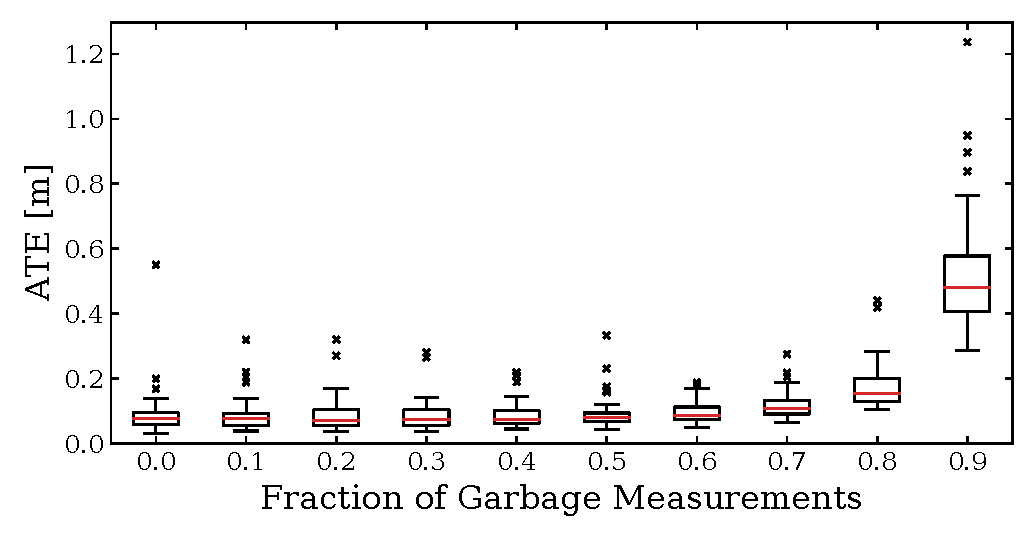
\includegraphics[page=1,width=.60\textwidth]{diagrams/sensor_noise.pdf}
    \caption[RobotWeb's robustness to garbage measurements]{A graph showing that the RobotWeb is robust to up to 70-80\% of ``garbage'' measurements, where faulty sensors report random measurements. ATE refers to the average Absolute Trajectory Error measured over 50 runs in an environment with 50 robots and 10 beacons running for 100 timesteps. Taken from \cite[Figure~5]{Robotweb}}
\end{figure}

Although the Robot Web is robust to many inter-robot sensors reporting random measurements, it is not robust to a bad actor which may instead report incorrect measurements designed to worsen the localisation of other members of the Robot Web. Possible attacks include but are not limited to:

\begin{enumerate}
    \item Sending messages with extremely low standard deviations, to lull others into a false sense of security.
    \item Sending these messages whilst assuming the identity of another robot.
    \item Sending these messages from many nonexistent robots, also known as a Sybil attack.
\end{enumerate}

\section{Security Issues}
In this section, we will discuss several general security issues that can arise in robot networks. We will focus on issues that affect the accuracy of a robot's internal model of the world. This excludes attacks which may result in an attacker gaining control over a robot, yet includes attacks performed by hijacked robots.

\subsection{Denial of Service} % Can go into more detail if necessary.
A denial of service attack seeks to deny service. In a robot network such as the Robot Web, this would prevent one or more robots from being able to access messages sent by their peers, and essentially cut them off from the network.

The simplest way for an attacker to perform a DoS attack is to use a signal jammer, which can be constructed using off-the-shelf equipment \cite{SignalJamming}. This would continuously transmit signals within the range of frequencies allowed by the communication medium, both interfering with and irrecoverably corrupting any messages sent. More sophisticated attackers may craft harder-to-detect jammer attacks by mimicking legitimate messages or only transmitting when it senses communication \cite{SignalJamming}. In addition to these, there exist a whole host of jamming attacks (and defences) targetting specific communication protocols.

Another form of a DoS attack would be to disconnect specific robots from the network, using the network protocol's existing defences. For example, by convincing others that the target is a bad actor, triggering their defences to remove the target from the network. % Kinda like a de-authentication attack, but not really since we're not sending explicit de-authentication frames to do this.

\subsection{Identity-Based Attacks}
% One class of attacks that could wreak havoc on robot networks are identity-based attacks; here a nonzero number of bad actors, claim false identities, which may or may not correspond to other robots in the network. The former is known as a spoofing attack, whilst the latter constitutes a Sybil attack.

Identity-based attacks can wreak havoc on robot networks. Using the model defined by Douceur \cite{SybilAttack}, we can describe a robot network as one consisting of $E$ entities (robots) each claiming at least one identity $i$ from the set of all identities $I$. When the network is under an identity-based attack, at least one of the following two properties will hold: % TODO maybe add the faulty/correct distinction
\begin{enumerate}
    \item Two entities, $e1, e2$ will present the same identity $i$
    \item The number of identities in $I$ will exceed the number of entities in $E$.
\end{enumerate}
If only the former holds, then the network is under a spoofing attack, whereas if only the latter holds, then the network is under a Sybil attack. Note: there is no guarantee that only one of these will hold at a time, and so we must be prepared to defend against both simultaneously.

\subsubsection{Spoofing Attacks}
Devices exchange information by sending packets or frames of data. For our purposes, we can ignore the differences between packets and frames, and use the terms interchangeably. Packets are used to encapsulate the data sent with relevant metadata, such as the source and destination IDs of the packet. This metadata is the main target of spoofing attacks.

In a spoofing attack, the attacker first finds the identity of a legitimate device, for example by first intercepting packets and then extracting the source ID from them. After this point, the attacker sends misleading packets impersonating the target. 

This can have several benefits for the attacker. Firstly, they could covertly inject misinformation into the network by impersonating an already trusted robot. Secondly, they could trigger defences in the network to flag target for misinformation and remove it.

\subsubsection{Sybil Attacks}
In a Sybil attack, the attacker will create many fake identities to gain undue influence on the network. In a robot network, this would allow them to indirectly influence the actions of victim robots. For example, one could lead two self-driving cars to conclude that their best course of action is to crash, by claiming many false identities would be hit if they were not to.

Douceur \cite{SybilAttack} proves Sybil attacks are always possible in distributed systems where there is no central arbiter of truth. They present and prove four lemmas about identities in large-scale distributed systems. The first two lemmas are concerned with entities which directly validate the identities presented to them, whilst the second two lemmas involve entities which rely upon other, potentially untrustworthy, identities for validation. The lemmas are as follows:

 %TODO lemma-ise

\begin{enumerate}
    \item If an attacker has $\rho$ times as many resources as the weakest entity, then they can successfully present up to $\lfloor\rho\rfloor$ distinct identities.
    \item If an entity doesn't validate all identities simultaneously, then an attacker can present an unbounded number of distinct identities.
    \item If an entity trusts $q$ other identities to validate an identity, then at least $f$ attackers are required to perform the attack, where $f >= q$ or the resources commanded by the attackers exceed $q + f$ times the weakest entity's resources.
    \item If all $c$ non-attackers don't coordinate when they validate identities, and an entity again trusts $q$ other identities for validation, then even a weak attacker can present $\lfloor\frac{c}{q}\rfloor$ identities.
\end{enumerate}

We plan to solve this problem by treating the physical world as a central arbiter of truth, albeit with some degree of error, due to imperfections in sensors.

\subsection{Physical Attacks}
Finally, since this thesis focuses on the security of robot networks, we will discuss the possibility of physical attacks on the system, and our limited ability to protect against them. We define a physical attack as any attempt to compromise the ability of a robot to perform its task. This includes colliding with the robot but also includes more subtle tactics, such as obscuring the robot's sensors. Physical attacks could also be used similarly to Sybil attacks, where several attackers would surround a robot and feed it misinformation. 

In this thesis, we will not attempt to protect against attacks where several robots would physically collide, since this would require heavy hardware modifications to existing robots. Instead, we will focus on occlusion attacks and physical Sybil attacks, at the very least allowing a robot to detect them.\\